The strength of a received signal measured at the receiver's antenna is received signal strength (RSS). Two main factors that determine RSS i.e. transmission power, the distance between the transmitter. 
A Location Verification System (LVS) based on RSS is interesting because of following factors\cite{yan14}: i) RSS is measurable in a wireless system as this is part of the box. So, no extra hardware is required therefore complexity is less and less cost ii) Many standards and specifications such as 802.11b require RSS to be available. iii) Sometimes RSS might be the only reliable information. For example, non-line-of-sight environments. RSS is highly co-related to transmitter or provers location. Localization or location estimation algorithms which are based on RSS first calculate the distances to the prover. These are done with the help of multiple reference points which act as acceptors or verifiers. These distances can be calculated because there is an inverse square relation between received signal power and the distance. The following expression shows this\cite{pu11}
\begin{equation}
    P_r \propto \frac{1}{d^2}
    \label{gm_delay}
\end{equation}

Here P is the received power from a distance d. This expression gives us the path loss by comparing difference between transmitted and received power. In practical applications the variations of path loss can be highly dependent on the environment.

Once RSSI distance and path loss model is estimated, lateration techniques can be used find the exact position of the prover. Lateration techniques can be used to estimate the position based on multiple reference locations i.e. the distances from different reference locations can be considered as radius of circles with center as the reference location. The unknown location is the intersection of all these circles.

\begin{figure}[htp]
    \centering
    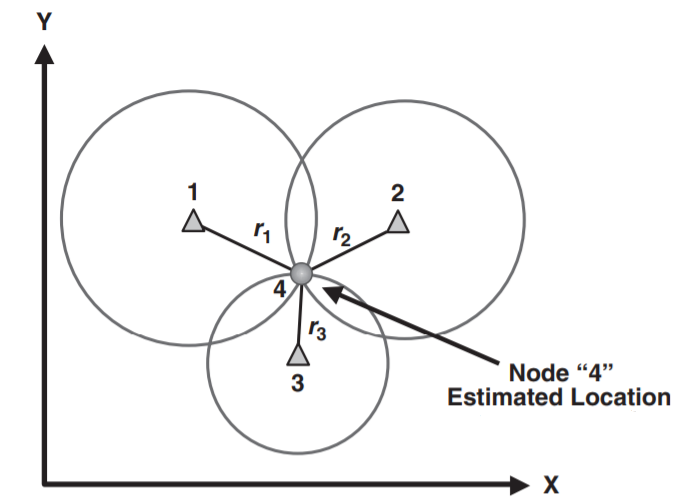
\includegraphics[width=7cm]{strength_trilat_pic.png}
    \caption{Location Estimation using Trilateration \cite{pu11}}
    \label{fig:strength_trilat_pic}
\end{figure}


\subsection{Limitations or disadvantages:} \label{rss_limitations}

Using RSS based location verification system is very tempting indeed because of the low cost, ready availability etc. as discussed above. But there are many limitations or problems. The main important problem is that the there is no control over transmit power. i.e. the attacker can act as a legitimate prover. So only weaker attackers can be detected. In the outdoor setting it is always advantageous to maintain the signal strength as high as possible to main a safety level of Link Quality Indicator, thus ensuring quality of our wireless communication. 
Another big limitation is that using such a system in an indoor environment is very hard. The main problems being multi path propagation, shadowing, and other noise sources makes location system based on RSS very hard to implement or in some cases completely unusable. 
\begin{figure}[htp]
    \centering
    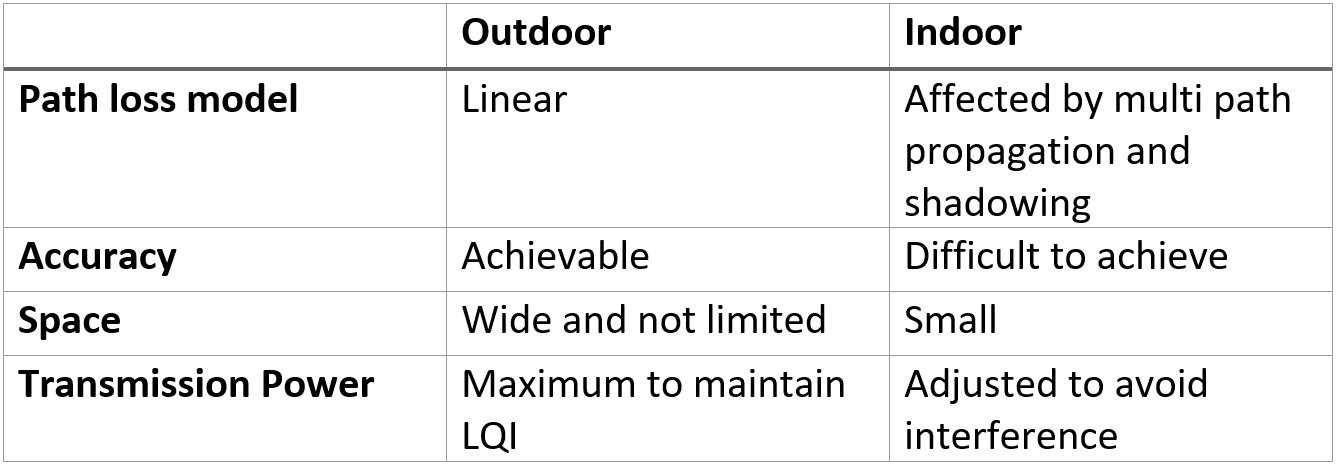
\includegraphics[width=9cm]{strength_comp_table.png}
    \caption{Outdoor vs Indoor \cite{pu11}}
    \label{fig:strength_comp_table}
\end{figure}
Finally, if mobility is involved i.e. if the wireless devices are mobile then an RSS base scheme alone becomes ineffective.


\subsection{Possible attacks and Current Methodologies} \label{rss_attacks}
RSS based systems are most vulnerable to spoofing attacks. Along with spoofing attackers try to use jamming and message replay to convince the verifiers.
There are different methods which try to detect spoofing and other attacks. Firstly, instead of using absolute signal strength Differential signal strength can be used. DRSS is difference between the signal strength values and the maximum value. In one of the detection mechanisms \cite{chenbook}, several access points (AP) at different fix locations are established which serve as sensors that measure RSS readings. A signalprint is constructed which is a vector of RSS at multiple access points. The idea is that signalprints are produced by wireless devices at different locations, which can be used to distinguish wireless devices located geographically apart. Different max and min matches and distributions are modelled based on which a RSS profile is established for each prover at different location. Any significant differences from these RSS patterns is considered as an attack. However, this method is computation intensive and when there is mobility involved it becomes ineffective.  Another verification method uses a set of covert base or verifiying stations. 

In coclusion RSS based location verification systems have many problems. These systems when combined with time difference of arrival (TDOA) perform better.


